\chapter{Referencial teórico}\label{cap:referencial}

Uma pergunta sobre animais que se alimentam de outros animais pode abrir uma discussão legítima sobre cadeias alimentares. A mesma temática pode aparecer em um pedido de instruções para ferir um animal. Se a regra de proteção considerar apenas as palavras presentes na pergunta, corre o risco de tratar os dois pedidos da mesma forma. Mesmo quando o sistema reconhece corretamente a intenção educativa, resta saber se o acervo permite responder à dúvida e se a explicação preserva o significado do conceito escolar. Essas três questões orientam a leitura da literatura sobre proteção infantil, geração com fontes e linguagem educativa.

\section{Seleção e alcance da literatura}

A busca narrativa realizada em 3 de novembro de 2026 reuniu trabalhos sobre modelos de linguagem, segurança de conteúdo para menores e recuperação de informação. Consideraram-se publicações de 2020 a 2026 em português ou inglês, além da Base Nacional Comum Curricular (BNCC), de 2018, por sua função curricular. As consultas combinaram termos como \textit{child}, \textit{guardrails}, \textit{educational chatbot} e seus correspondentes em português. A seleção privilegiou estudos com método identificável, descrições originais das arquiteturas e documentos oficiais. As consultas e os critérios estão registrados em \nolinkurl{avaliacao/BUSCA_NARRATIVA.md}.

Uma consulta complementar reuniu estudos primários sobre recuperação vetorial, avaliação de citações e compreensão de relações entre ideias no ensino fundamental. A seleção é intencional. Permite confrontar métodos e justificar o recorte do projeto, mas não permite estimar a frequência de falhas em chatbots infantis nem afirmar que inexistem trabalhos semelhantes em português brasileiro.

\section{Proteção infantil e interpretação da intenção}

Wang et al. (2022) examinam a correspondência entre princípios gerais de inteligência artificial (IA) e orientações de design apropriado à idade. Sua contribuição é situar as necessidades das crianças entre os critérios de projeto desde a concepção do sistema. Para o GuardKids, isso afeta tanto a decisão de responder quanto a forma de fazê-lo. Se o estudante relata que sofreu uma ofensa, repetir o conteúdo ofensivo ou pedir dados para identificar os envolvidos é desnecessário para oferecer uma orientação de cuidado. Bloquear o relato sem reconhecer o pedido de ajuda também pode deixar a necessidade do estudante sem atendimento.

Rath et al. (2025) constroem perfis infantis com interesses e características distintas e os empregam para avaliar seis modelos de linguagem. Os autores identificam falhas em categorias de conteúdo especialmente relevantes para menores. Já Khoo, Chua e Shong (2025) partem de um estudo de caso em ambiente escolar e propõem o MinorBench para examinar se modelos recusam solicitações inadequadas. Enquanto Rath et al. variam as características do interlocutor simulado, o MinorBench organiza a avaliação em torno de situações de risco e da resposta do modelo a elas. As abordagens se complementam, mas respondem a perguntas diferentes: que riscos aparecem quando muda o perfil considerado e que solicitações recebem o tratamento esperado?

O GuardKids fixa um perfil fictício de nove anos, correspondente ao quarto ano, e formula casos próprios em português brasileiro. Fixar o perfil permite comparar duas explicações dirigidas ao mesmo interlocutor. Em contrapartida, deixa fora da comparação as diferenças de repertório entre crianças, inclusive entre as da mesma idade. A faixa de sete a onze anos designa o público pretendido. Os casos do projeto não são uma tradução validada do MinorBench, e o estudo não contou com participantes infantis.

O guia brasileiro de classificação indicativa fornece descritores para analisar conteúdo em seu contexto de apresentação (Brasil, 2025). Sua contribuição para a PoC é oferecer vocabulário para discutir risco. A decisão de um chatbot exige ainda interpretar o que o usuário solicita e o que uma resposta tornaria possível. Uma descrição não gráfica de predação e uma instrução para causar dano podem mencionar o mesmo animal, mas somente a segunda pede auxílio para feri-lo. O uso dos descritores é uma adaptação de projeto. O chatbot não recebeu classificação indicativa oficial.

A Figura~\ref{fig:contexto} mostra uma consequência dessa distinção. Diante de um relato de intimidação, pode caber uma orientação de cuidado. Diante de um pedido para humilhar um colega, pode caber o bloqueio. Se a pergunta for educativa, a decisão seguinte é documental: verificar se o acervo contém elementos para respondê-la. Uma mensagem de apoio insuficiente comunica um limite das fontes, e seu sentido para o estudante é diferente do de uma recusa por risco.

\begin{figure}[htbp]\centering
\caption{Análise contextual da intenção e do tratamento da solicitação}\label{fig:contexto}
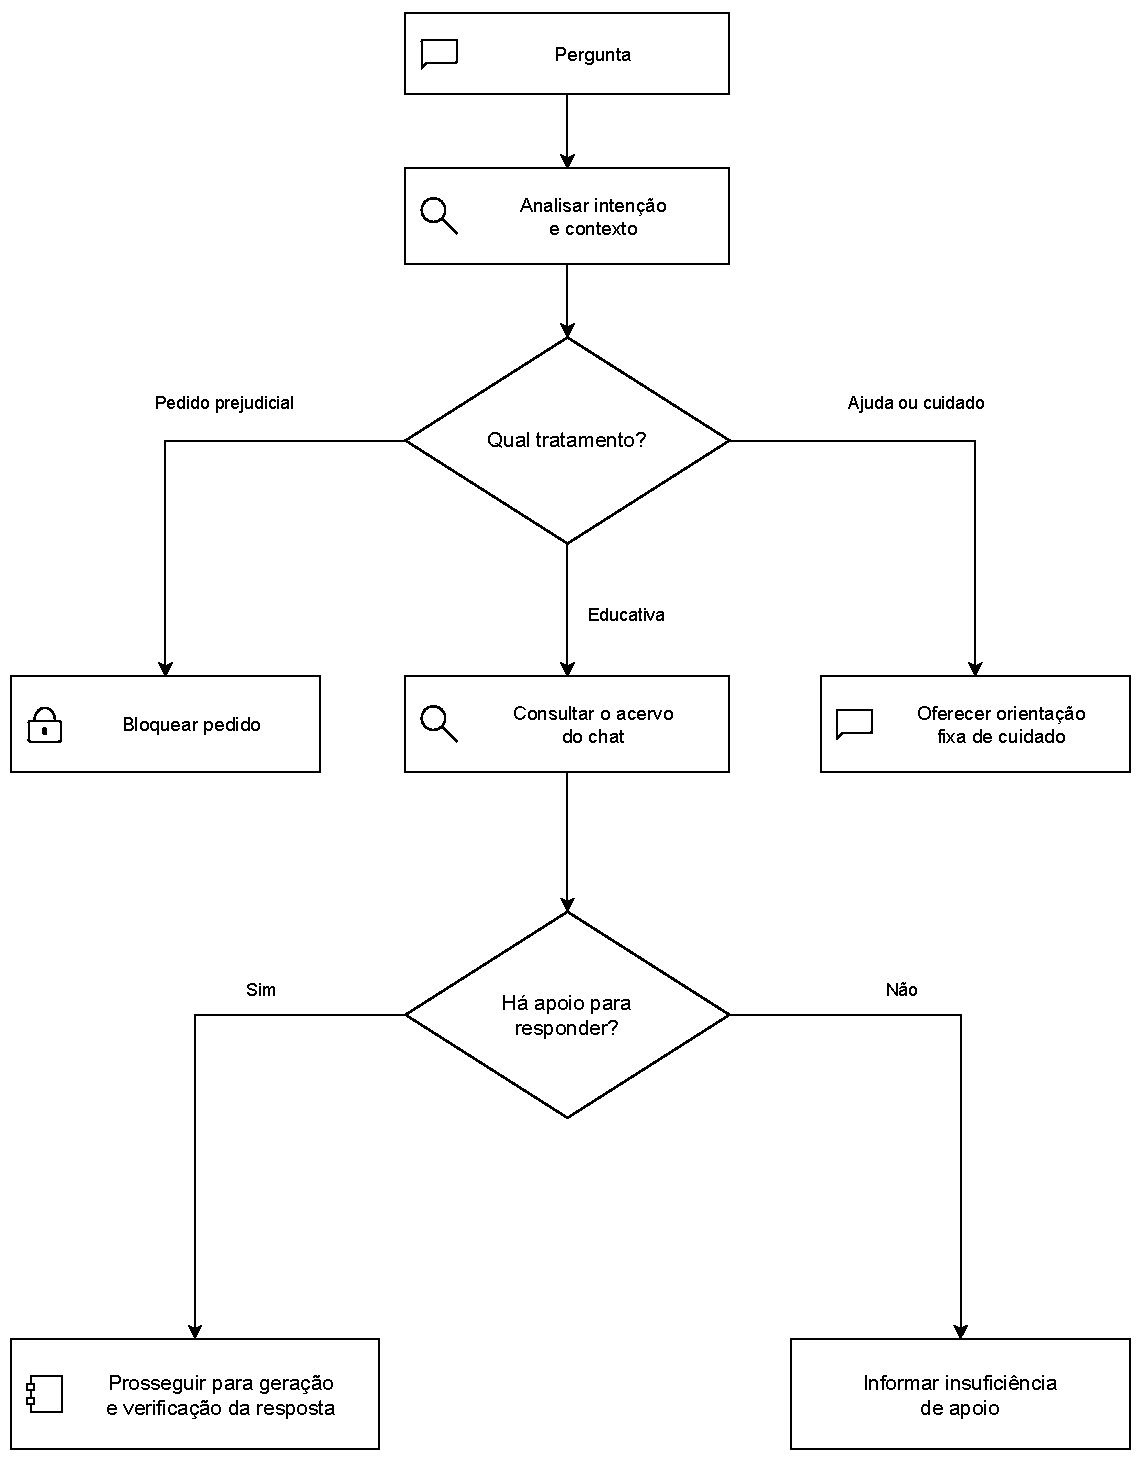
\includegraphics[width=\textwidth,height=0.82\textheight,keepaspectratio]{diagramas/pdf/02_Analise_contextual.pdf}
\fonte{Elaboração própria com base nos descritores de Brasil (2025) e na regra da PoC.}
\end{figure}

\section{Guardrails de entrada e de saída}

Neste trabalho, \textit{guardrails} são regras e verificações que determinam quando uma aplicação pode prosseguir, deve substituir uma resposta ou precisa interromper o processamento. A política expressa o tratamento pretendido. O classificador atribui uma categoria a uma mensagem concreta. A ação resulta da aplicação da política ao que foi reconhecido. Separar esses elementos ajuda a localizar um erro: uma regra pode prever cuidado em pedidos de ajuda e, ainda assim, produzir um bloqueio se o classificador interpretar o relato como agressão.

Rebedea et al. (2023) apresentam o NeMo Guardrails como uma ferramenta para programar restrições ao comportamento de aplicações conversacionais. Inan et al. (2023) abordam outro componente do problema com o Llama Guard, um modelo instruído a classificar entradas e respostas segundo categorias de segurança. O primeiro trabalho trata da organização dos controles na aplicação; o segundo trata da atribuição de um julgamento a um texto. A PoC toma dessas abordagens a separação entre política, classificação de entrada e verificação de saída. Sua implementação usa instruções locais e respostas estruturadas do Qwen3:8b.

A diferença entre entrada e saída é substantiva. Uma pergunta escolar aceitável pode levar o gerador a acrescentar um detalhe inadequado que o estudante não pediu. A classificação da entrada não examina esse detalhe, pois ele só aparece após a geração. Já uma resposta bloqueada por erro de classificação pode privar o estudante de uma explicação legítima. Por isso, a avaliação deve observar tanto a permissão indevida quanto a recusa indevida. Contar bloqueios, isoladamente, favoreceria até um sistema que recusasse todas as perguntas. Uma falha técnica tampouco merece crédito como proteção bem-sucedida: ela informa que a tentativa não pôde ser concluída.

\section{Recuperação de informação e sustentação das respostas}

Lewis et al. (2020) combinam a informação incorporada aos parâmetros de um modelo com uma memória externa de documentos recuperáveis. Essa formulação da geração aumentada por recuperação (\textit{retrieval-augmented generation}, RAG) permite condicionar a geração a passagens relacionadas à pergunta. O GuardKids adota o princípio da consulta a uma memória externa, com um acervo selecionado por chat. Quando a fonte é conhecida, o avaliador pode voltar ao trecho utilizado e perguntar quais afirmações da explicação encontram apoio nele.

A recuperação densa representa perguntas e passagens por vetores e usa sua proximidade para ordenar candidatos. Chen et al. (2024) descrevem o BGE-M3, que admite diferentes formas de recuperação. A PoC utiliza sua representação densa e restringe a seleção aos trechos do chat escolhido. Considere uma pergunta sobre o tempo de decomposição de uma folha. Uma passagem que explica o papel dos fungos pode ser a mais próxima da pergunta e, ainda assim, não informar prazo algum. O escore de similaridade serve à seleção de passagens. A suficiência depende da relação entre o que a pergunta exige e o que o trecho efetivamente afirma.

Há, portanto, três verificações distintas. Primeiro, é preciso saber se o acervo autorizado contém material para responder. Segundo, verifica-se se a busca recuperou esse material. Terceiro, compara-se a resposta com as passagens citadas. Uma falha na busca pode levar o sistema a declarar insuficiência apesar da existência de apoio. No sentido inverso, recuperar a passagem adequada não impede o modelo de acrescentar uma recomendação ausente da fonte. Distinguir essas situações permite localizar o problema antes de alterar o acervo, o mecanismo de busca ou as instruções de geração.

Gao et al. (2023) tornam essa distinção observável ao avaliar separadamente fluência, correção e qualidade das citações em sistemas que respondem com fontes. Para o GuardKids, uma referência válida identifica qual trecho foi consultado. Julgar a sustentação exige ler esse trecho e verificar se ele apoia cada afirmação relevante, inclusive exemplos. Uma frase pode ser plausível ou mesmo factualmente correta e continuar sem apoio no acervo delimitado. Também pode reproduzir fielmente uma fonte que contenha um erro. Daí a necessidade de avaliar tanto as respostas quanto a qualidade do material selecionado.

O mesmo modelo participa da geração e da verificação semântica no protótipo. Se ambas as chamadas admitirem uma inferência indevida, a segunda pode confirmar o acréscimo feito pela primeira. A verificação automática acrescenta uma oportunidade de detectar falhas. O confronto independente entre afirmação e fonte continua necessário para estimar quantas respostas liberadas atendem ao critério de sustentação.

\section{Clareza da explicação e recorte curricular}

A clareza de uma explicação envolve a relação entre suas ideias. Dizer que fungos e bactérias decompõem restos de seres vivos oferece ao aluno um ponto de partida. Para explicar a importância desse processo, é preciso também mostrar como a liberação de nutrientes se relaciona com sua disponibilidade no ambiente. Em texto escolar, dividir a resposta em frases curtas pode facilitar a leitura local e, ao mesmo tempo, deixar implícita a relação causal que motivou a pergunta.

Volodina e Weinert (2020) investigaram a compreensão de conectivos em estudantes do ensino primário na Alemanha, acompanhando duas coortes, uma do segundo ao terceiro ano e outra do terceiro ao quarto ano, articuladas em um desenho sequencial de coortes. O estudo trata de como os alunos compreendem palavras que expressam relações entre ideias, como causa ou contraste. Para esta pesquisa, oferece uma razão para examinar se a explicação explicita corretamente essas relações. Seus dados, obtidos em alemão em tarefas específicas, não estabelecem qual estilo de resposta funciona melhor para uma criança brasileira.

No estilo Direto, o desafio é preservar a relação essencial sem exigir que o leitor conheça um termo que a própria resposta deveria explicar. No Passo a passo, a divisão em etapas e a presença de um exemplo podem tornar a relação mais explícita, mas aumentam o número de afirmações que precisam ser verificadas. Em um mapa hipotético, por exemplo, uma cor pode representar uma cidade se a legenda assim o indicar. Apresentar a mesma associação como convenção de todos os mapas produziria uma generalização injustificada. O que interessa comparar é se o exemplo esclarece o conceito, respeita a fonte e responde à dúvida. A preferência de um avaliador por uma explicação e a compreensão efetiva por uma criança exigem evidências diferentes.

A BNCC situa o recorte inicial de Ciências em dois objetivos do quarto ano. A habilidade EF04CI04 trata de cadeias alimentares simples e do papel do Sol como fonte primária de energia. A EF04CI06 aborda a participação de fungos e bactérias na decomposição e a importância ambiental desse processo (Brasil, 2018, p.~339). A Tabela~\ref{tab:curriculo} identifica o material disponível para tratar desses objetivos. Esse vínculo explica por que uma pergunta sobre predação pode ser legítima naquele contexto escolar e por que sua resposta precisa preservar a relação ecológica estudada.

\begin{table}[htbp]\centering\small\SingleSpacing
\caption{Correspondência curricular do recorte inicial de Ciências}\label{tab:curriculo}
\begin{tabularx}{\textwidth}{L{2.1cm} Y Y L{1.8cm}}
\toprule Habilidade & Objetivo de explicação & Trechos recuperáveis & Famílias históricas \\\midrule
EF04CI04 & Relacionar alimentação, produtores e consumidores & \nolinkurl{trilhas2021-p154-1}; \nolinkurl{sp2024-p8-1}; \nolinkurl{sp2024-p9-1} & L01, L02, P01--P03 \\
EF04CI06 & Explicar decomposição e retorno de nutrientes & \nolinkurl{sp2024-p13-1}; \nolinkurl{sp2024-p27-1} & L03 \\
\bottomrule\end{tabularx}\fonte{Elaboração própria; BNCC e recortes do índice utilizado no lote de desenvolvimento.}
\end{table}

Os cinco trechos de Ciências permitem tratar desses conceitos dentro de limites identificáveis. Uma pergunta sobre a quantidade diária de alimento de uma espécie, por exemplo, pode estar relacionada à cadeia alimentar sem encontrar resposta no material selecionado. Em História, Geografia e Geral, o acervo contém uma síntese experimental por chat. A vinculação curricular documentada para Ciências não se estende automaticamente a esses outros espaços.

\section{Síntese e implicações para a pesquisa}

A Tabela~\ref{tab:trabalhos} organiza as contribuições da literatura segundo a decisão que cada uma fundamenta. Dessa comparação resulta o recorte do TCC I: examinar, em perguntas educativas e de proteção, se a aplicação reconhece a intenção, consulta fontes pertinentes e entrega uma explicação que possa ser julgada quanto à correção, à sustentação e à clareza.

\begin{table}[htbp]\centering\small\SingleSpacing
\caption{Decisões do GuardKids fundamentadas na literatura}\label{tab:trabalhos}
\begin{tabularx}{\textwidth}{L{3.2cm} Y Y}
\toprule Estudos & Evidência ou contribuição & Decisão para o GuardKids \\\midrule
Wang et al. (2022); Rath et al. (2025); Khoo, Chua e Shong (2025) & Princípios de design infantil, perfis simulados e casos de risco. & Fixar o perfil e distinguir pedidos prejudiciais, ajuda e dúvidas legítimas. \\
Rebedea et al. (2023); Inan et al. (2023) & Controles programáveis e classificação de entradas e saídas. & Examinar em qual etapa ocorreu uma intervenção e se ela era adequada. \\
Lewis et al. (2020); Chen et al. (2024); Gao et al. (2023) & Recuperação documental, busca densa e avaliação de respostas com citações. & Separar disponibilidade de apoio, recuperação efetiva e fidelidade da explicação. \\
Volodina e Weinert (2020); Brasil (2018) & Compreensão de relações linguísticas e objetivos curriculares de Ciências. & Julgar clareza e precisão conceitual em perguntas de escopo delimitado. \\
\bottomrule\end{tabularx}\fonte{Elaboração própria.}
\end{table}

Para que a comparação entre estilos tenha uma interpretação definida, a mesma pergunta deve ser submetida aos dois estilos com perfil, política e acervo mantidos constantes. As mensagens fixas de cuidado podem coincidir nas duas condições; a comparação de clareza ganha sentido sobretudo nos pares em que há explicações educativas. Esse desenho sustenta o protocolo do Capítulo~\ref{cap:metodo}. Seu alcance é a análise do comportamento do artefato e dos textos produzidos, com avaliação humana de conteúdo prevista para etapa posterior.
